\iflanguage{english}
{\chapter{Verwandte Arbeiten}}
{\chapter{Related Work}}
\label{sec:related}

This chapter provides a literature review of key developments in 3D human reconstruction and texture estimation. I will begin by discussing explicit reconstruction methods, which rely on parametric models, followed by implicit approaches that capture surface geometry in a more flexible method. After that, I will dive into texture estimation, introducing methods that directly estimate or synthesize human textures. Lastly, I highlight the limitations of current approaches and clarify my research gap and motivation for HRHumanTex.

\section{Explicit 3D Human Reconstruction}

Explicit reconstruction methods represent the human body using parameterized mesh models such as SMPL~\cite{SMPL:2015}, SMPL-X~\cite{SMPL-X:2019}, and STAR~\cite{STAR:2020}. These models provide low-dimensional control over body shape and pose, and have become widely adopted due to their efficiency and compatibility with standard rendering pipelines. For example, SMPL’s linear blend skinning makes it well-suited for pose-dependent deformation modeling. 

A range of recent works, such as HMR~\cite{kanazawaHMR18}, SPIN~\cite{kolotouros2019spin}, and PARE~\cite{Kocabas_PARE_2021} have proposed end-to-end neural networks could estimate body shape, pose, and often camera parameters from monocular images. PIXIE~\cite{PIXIE:2021} and ROMP~\cite{ROMP} further integrate facial and hand estimation into unified pipelines, enabling more holistic full-body reconstructions. Figure~\ref{fig:romp} shows the overview of ROMP, which I also used in my rendering-based evaluation and optimization section in HRHumanTex.

\begin{figure}[h]
    \centering
    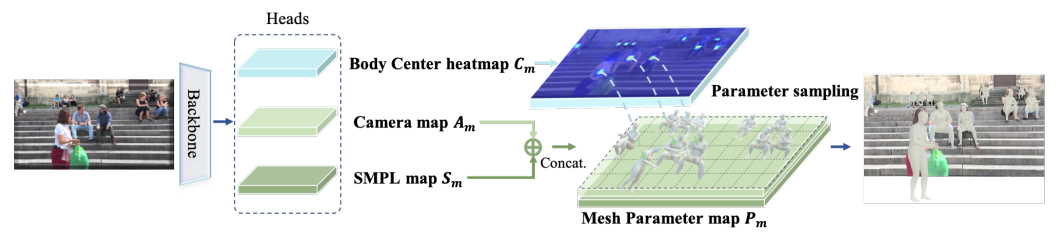
\includegraphics[width=0.95\textwidth]{fig/romp.png}
    \caption{An overview of Monocular, One-stage, Regression of Multiple 3D People(ROMP).~\cite{ROMP}}
    \label{fig:romp}
\end{figure}

While these methods enable controllable and clean mesh-based representation, they rely heavily on accurate 2D keypoint or segmentation supervision and often struggle with modeling loose clothing, hair, or non-body accessories due to the fixed mesh topology. These limitations have motivated the development of implicit methods that can model arbitrary geometries more flexibly. By the way, most explicit human reconstruction methods (such as HMR, SPIN, PARE, ROMP, etc.) only reconstruct the geometry (shape + pose, sometimes include camera parameters) and without addressing surface appearance or texture, this also confirms my thesis work, how important it is to be able to successfully estimate texture from images.


\section{Implicit 3D Human Reconstruction}

Recent advancements in implicit representations have enabled high-fidelity reconstruction of clothed human bodies from sparse inputs. Unlike parametric models, implicit methods model the surface as a continuous function and offer better flexibility in capturing arbitrary topology, overcome the topological rigidity of mesh-based models.

PIFu and PIFuHD~\cite{saito2019pifu, saito2020pifuhd} introduced pixel-aligned implicit functions that estimate occupancy values using per-pixel features sampled along camera rays. PIFuHD further enhances the fidelity of visual details via multi-scale information extraction and hierarchical learning. These methods implicitly reconstruct both geometry and texture, can recover both geometry and coarse texture cues, even in occluded regions.

ICON~\cite{xiu2022icon} builds upon this framework by combining implicit surface estimation with SMPL model guidance. It predicts both occupancy fields and surface normals while incorporating visibility-aware feature extraction. A refinement loop adjust the initial SMPL predictions, improving robustness to pose errors and enabling better recovery of loose clothing and fine wrinkles.

More recently, TeCH~\cite{huang2024tech} demonstrates a novel integration of generative priors and optimization. By combining DreamBooth-style appearance conditioning with text-guided geometry generation and latent score distillation sampling(LSDS), TeCH produces high-fidelity reconstruction of both shape and texture from limited views. Figure~\ref{fig:tech}
shows the overview of TeCH workflow.
\begin{figure}[h]
    \centering
    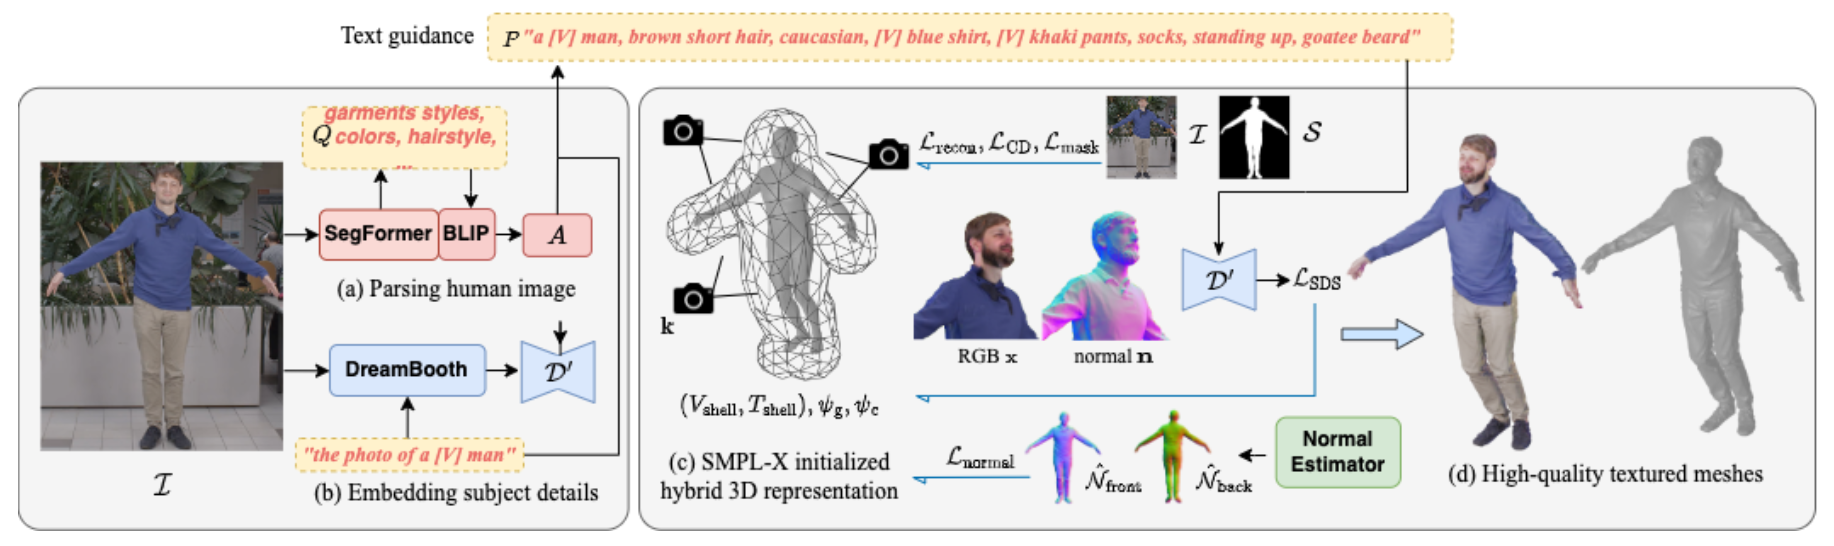
\includegraphics[width=0.95\textwidth]{fig/tech.png}
    \caption{TeCH: Text-guided Reconstruction of
Lifelike Clothed Humans Overview.~\cite{huang2024tech}}
    \label{fig:tech}
\end{figure}

Despite their flexibility and ability to recover fine-scale detail, implicit methods face practical challenges such as high computational cost, slow inference speed, and difficulties in recovering high-resolution texture information or explicit mesh outputs for downstream applications, such as animations. 



\section{Human Texture Estimation: A Survey}

Estimating realistic full-body textures from limited visual input remains a challenging task due to self-occlusions, pose variation, and the difficulty of preserving high-frequency details. This section reviews recent methods that aim to estimate complete UV texture maps from monocular images or sparse views.

\subsection{SMPLitex: Diffusion-based 3D Human Texture Estimation}

SMPLitex~\cite{casas2023smplitex} is the first method to use latent diffusion models (LDMs)~\cite{rombach2021highresolution} for generating complete 3D human UV textures from single RGB images. The key idea is to reformulate the 3D human appearance estimation problem as a conditional image generation task in UV space, taking advantage of the 2D nature of UV parameterization.

The backbone of SMPLitex is a latent diffusion model, which operates on a variational autoencoder (VAE)-encoded latent space $\mathbf{z}_t$ and is trained to iteratively denoise it over $T$ steps, optimizing the following objective:
\begin{equation}
\mathcal{L}_{\text{diff}} = \mathbb{E}_{\mathbf{z}_t, c, t, \varepsilon \sim \mathcal{N}(0,1)} \left[\left\| \varepsilon - \varepsilon_\theta(\mathbf{z}_t, c, t) \right\|_2^2\right],
\end{equation}
where $c$ can be a conditioning signal such as partial texture or text.

To condition the generation on real input images, SMPLitex employs DensePose~\cite{wu2019detectron2} and SGHM~\cite{chen2022sghm} to compute pixel-to-surface correspondences $\mathbf{d}$ and a human mask $\mathbf{s}$, which results in a partial UV map:
\begin{equation}
\mathbf{u}_{\text{part}} = \Pi(\mathbf{x}, \mathbf{d} \odot \mathbf{s}),
\end{equation}
where $\Pi$ is the UV projection operator. The model is then guided to inpaint the full texture $\mathbf{u}_{\text{full}}$ from this partial texture $\mathbf{u}_{\text{part}}$.

SMPLitex demonstrates high-quality texture estimation and completion, enables novel applications such as text-conditioned texture generation and inpainting. However, its output resolution is limited to $512 \times 512$, when generalizing to higher resolutions always produces serious hallucinations.


\subsection{Texformer: Transformer-Based Texture Estimation}

\begin{figure}[h]
    \centering
    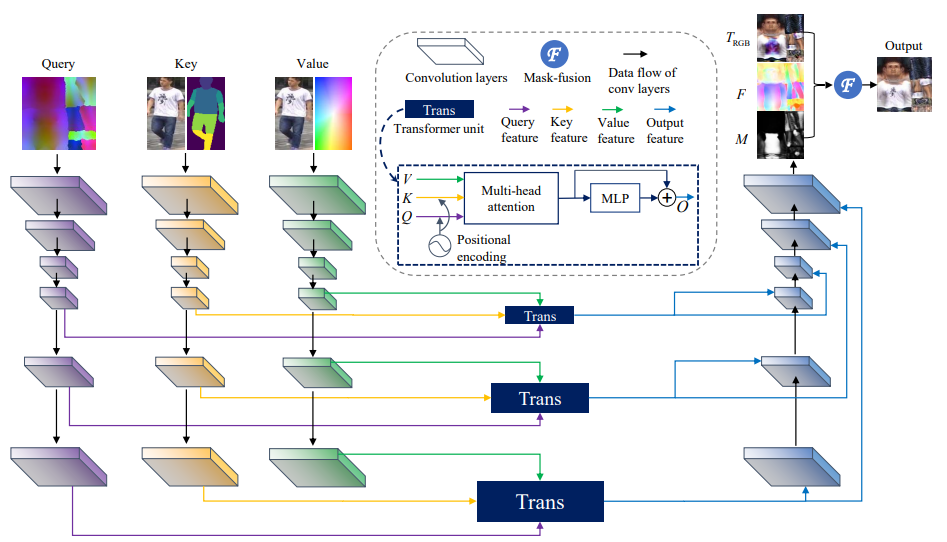
\includegraphics[width=0.95\textwidth]{fig/texformer.png}
    \caption{Texformer: 3D Human Texture Estimation from a Single Image with Transformers.~\cite{xu2021texformer}}
    \label{fig:texformer}
\end{figure}

Texformer~\cite{xu2021texformer} introduces a Transformer-based architecture for estimating full-body uv textures from a single input image. It reformulates the texture regression task as a Query-Key-Value attention problem between the 2D image space and the UV texture space. Figure~\ref{fig:texformer} shows the architecture of Texformer.

\paragraph{Core Method.}
\begin{itemize}
    \item \textbf{Query:} Encodes UV coordinate using 3D body coordinates derived from SMPL, these are projected to UV space and embedded through a \ac{CNN}.
    \item \textbf{Key:} Combines a 2D part segmentation map (from a human parsing model) with the input image, enabling alignment between image features and UV positions.
    \item \textbf{Value:} Concatenation of RGB input image and image-space texture flow field, enabling the model to represent not only color information but also spatial correspondences between UV locations and image pixels.
\end{itemize}

The Transformer module computes UV-space output features $O \in \mathbb{R}^{vu \times c}$ using a multi-head attention mechanism followed by a residual Multi-Layer-Perceptron (MLP) block$f_{\text{res-MLP}}$:
\begin{equation}
O = f_{\mathrm{res\text{-}MLP}}\left( f_{\mathrm{Attn}}(Q + E_Q, K + E_K, V) \right),
\end{equation}
where $E_Q, E_K$ are positional encodings.

To reduce memory cost for high-resolution attention, Texformer introduces a \textbf{low-rank attention (LoRA)} formulation:
\begin{equation}
f_{\mathrm{LoRA}}(\tilde{Q}, \tilde{K}, \tilde{V}) = \frac{1}{\alpha} \tilde{Q} \tilde{K}^{\top} \tilde{V},
\end{equation}
This approximation avoids the use of softmax and allows more efficient computation through matrix reordering.

\paragraph{Mask Fusion for Output.}
Texformer outputs both an RGB UV texture $T_{\mathrm{RGB}}$ and a texture flow $F$. A learned fusion mask $M$ is used to blend these two:
\begin{equation}
T = M \odot f_{\text{sample}}(F, I) + (1-M) \odot T_{\mathrm{RGB}},
\end{equation}
where $f_{\text{sample}}$ denotes bilinear sampling from input image $I$.

\paragraph{Loss Design.}
Texformer introduces a multi-term loss to address color fidelity and facial structure:
\begin{itemize}
    \item \textbf{ReID loss:} Encourages appearance consistency with the input image by a person re-identification network as a perceptual guide.
    \item \textbf{Part-style loss:} Applies Gram matrix style matching to individual body parts, helping resolve inconsistencies across segmented regions.
    \item \textbf{Face-structure loss:} Uses structure similarity to align generated facial textures with synthetic ground truth examples.
\end{itemize}
The total loss is:
\begin{equation}
\mathcal{L} = w_1 \mathcal{L}_{\mathrm{ReID}} + w_2 \mathcal{L}_{\mathrm{style}} + w_3 \mathcal{L}_{\mathrm{face}}.
\end{equation}
where $w_1$,$w_2$,$w_3$ are weighting terms balancing the contributions of each loss component.

\paragraph{Summary.}
Texformer achieves high-fidelity UV map estimation by combining Transformer-based attention, flow-guided sampling, and region-specific fusion. Its multi-scale architecture and loss design improve visual details in both visible and occluded regions of the body.

\subsection{HPBTT: Human Parsing Based Texture Transfer}

\begin{figure}[h]
    \centering
    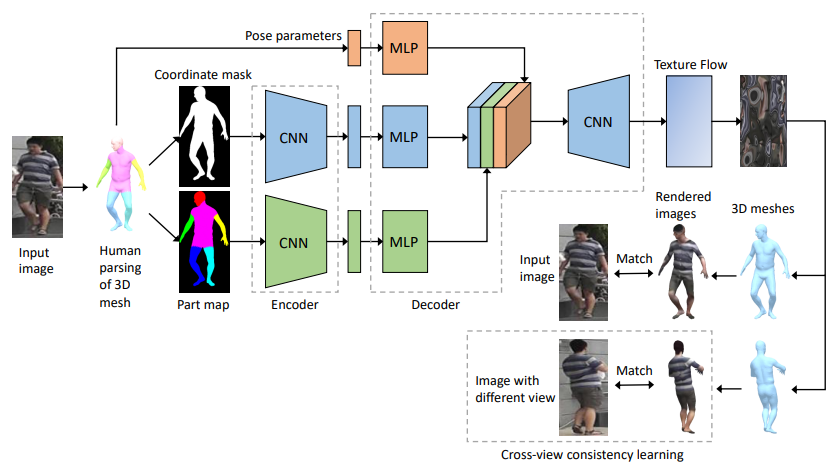
\includegraphics[width=0.95\textwidth]{fig/hpbtt.png}
    \caption{Overview of Human Parsing Based Texture Transfer from Single
Image to 3D Human via Cross-View Consistency.~\cite{zhao2020human}}
    \label{fig:hpbtt}
\end{figure}

HPBTT~\cite{zhao2020human} introduces a framework for estimating 3D human textures from a single image, without relying on 3D ground-truth supervision. The method builds upon two key ideas: semantic-aware texture flow prediction and a novel cross-view consistency loss. By incorporating human parsing and leveraging pose-aware cues, HPBTT achieves dense texture transfer from image space to UV space with improved generalization to unseen body regions.

\paragraph{Semantic-Driven Texture Flow Prediction.}
Rather than directly generating RGB textures, HPBTT predicts a texture flow field $\mathbf{F} \in \mathbb{R}^{H_{uv} \times W_{uv} \times 2}$ to sample from the input image:
\begin{equation}
\mathbf{I}^{uv} = g(\mathbf{I}; \mathbf{F}),
\end{equation}
where $g$ is a bilinear sampling function. The model input is not the original image. Instead, it uses a two-part semantic parsing map:

$\mathbf{I}^{\text{mask}}$: a coordinate mask encoding body shape.

$\mathbf{I}^{\text{part}}$: a part segmentation map using distinct RGB encodings to capture human pose.

Each input is processed through a separate convolutional encoder, and a decoder jointly conditions on the shape, pose features, and SMPL-estimated pose vector $\theta$ to predict $\mathbf{F}$:
\begin{equation}
\mathbf{F} = f_{\text{dec}}\left([\; f^{1}_{\text{enc}}(\mathbf{I}^{\text{mask}}), f^{2}_{\text{enc}}(\mathbf{I}^{\text{part}}), \theta \;] \right).
\end{equation}

\paragraph{Cross-View Consistency Supervision.}
To supervise unseen body parts, HPBTT introduces a cross-view perceptual loss: for two views $\mathbf{I}_1, \mathbf{I}_2$ of the same subject, textures are transferred and rendered onto each other's mesh, ensuring mutual consistency:
\begin{equation}
\mathbf{I}^{\text{rend}}_{1 \rightarrow 2} = R(M_2, \mathbf{I}^{uv}_1), \quad \mathbf{I}^{\text{rend}}_{2 \rightarrow 1} = R(M_1, \mathbf{I}^{uv}_2).
\end{equation}
The final loss combines view-consistent perceptual supervision with total variation regularization over $\mathbf{F}$ to encourage smooth sampling, the complete objective is:
\begin{equation}
\mathcal{L} = \mathcal{L}_{\text{tex}} + \lambda \mathcal{L}_{\text{tv}}.
\end{equation}

\paragraph{Summary.}
HPBTT’s main contribution lies in using semantic parsing to guide texture transfer and replacing direct supervision with a cross-view consistency loss. This formulation enables the model to learn from single-view images while handling occlusions and pose variations effectively. Compared to prior silhouette- or flow-based approaches, HPBTT offers a more semantically informed and geometrically robust solution to monocular image texture estimation.


\subsection{360-Degree Textures of People from a Single Image}

This work by Verica Lazova et al.~\cite{lazova2019360} presents a complete pipeline for reconstructing textured 3D human models from a single image. Their method directly operates in the SMPL UV space and jointly predicts three components: a full texture map, a clothing segmentation map, and a displacement map for geometry refinement. 

To train their model, they register the SMPL mesh to 4541 3D scans of clothed people through non-rigid deformation. The SMPL model is extended with learned vertex offsets $\mathbf{D}$ to capture clothing and hair. These offsets are added to the template mesh to deform the surface beyond the limitations of the base model:
\begin{equation}
M(\boldsymbol{\theta}, \boldsymbol{\beta}, \mathbf{D}) = W(\mathbf{T}_\mu + B_s(\boldsymbol{\beta}) + B_p(\boldsymbol{\theta}) + \mathbf{D}, J(\boldsymbol{\beta}), \boldsymbol{\theta}, \mathbf{W}).
\end{equation}

The technical framework consists of three innovation modules:  

(1) Texture Completion Module: Using DensePose~\cite{wu2019detectron2} to extract partial textures, followed by a conditional GAN~\cite{goodfellow2014generativeadversarialnetworks}-based inpainting network to generate full UV textures. The loss function includes adversarial, pixel-wise reconstruction, perceptual, and DSSIM components.  

(2) Semantic Segmentation Module: A separate image-to-image model predicts complete garment segmentation in UV space. This output serves as an additional control signal for geometry prediction and supports applications such as re-texturing or part-wise editing.  

(3) Displacement Prediction Module: Based on the outputs of the first two modules, the generator learns vertex displacement parameters to generate 3D clothing geometry with rich details on the base human body model.

This approach has a significant advantage: it uses a consistent UV-space representation across all tasks (texturing, segmentation, and displacement). This facilitates model coordination and supports pose-invariant learning. This design enables downstream applications, including 3D virtual image generation, clothing editing, and virtual fitting, without requiring explicit multi-view or 3D supervision during inference. Figure~\ref{fig:360degree} shows this architecture.


\begin{figure}[h]
    \centering
    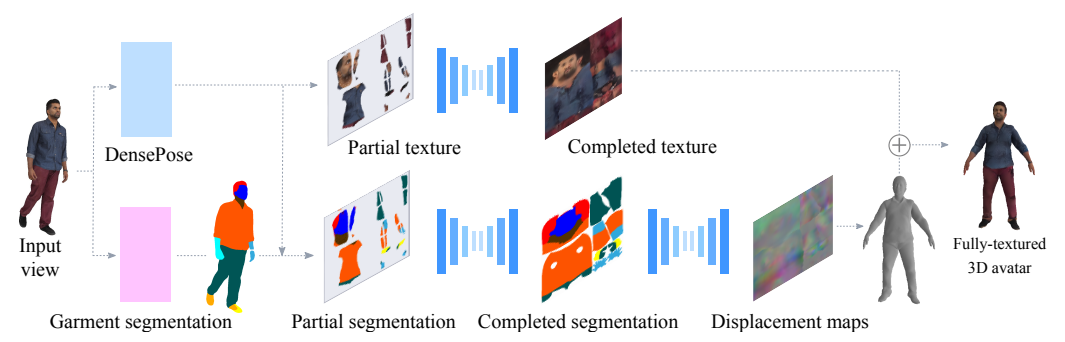
\includegraphics[width=0.95\textwidth]{fig/360degree.png}
    \caption{360-Degree Textures of People in Clothing from a Single Image Architecture.~\cite{lazova2019360}}
    \label{fig:360degree}
\end{figure}

\subsection{Learning to Reconstruct People in Clothing from a Single RGB Camera}

The method ~\cite{alldieck2019learningreconstructpeopleclothing} presents a fast and practical framework for reconstructing detailed 3D models of clothed humans from a few monocular RGB video frames, called Octopus. The system is designed for efficiency, completing reconstructions in under 10 seconds while recovering detailed geometry of the body, hair, and clothing. To achieve this, this paper proposes a CNN-based architecture that directly predicts SMPL+D parameters from a small set of frames. The predicted shape can then be refined by instance-specific optimization.

The shape representation builds upon the SMPL model~\cite{SMPL:2015}, extended by learnable per-vertex offsets $\mathbf{D}$ to model clothing and hair. Given the estimated shape $\boldsymbol{\beta}$ and pose $\boldsymbol{\theta}$, the final mesh is obtained through standard linear blend skinning:

\[
M(\boldsymbol{\beta}, \boldsymbol{\theta}, \mathbf{D}) = W\left( \mathbf{T} + B_s(\boldsymbol{\beta}) + B_p(\boldsymbol{\theta}) + \mathbf{D}, J(\boldsymbol{\beta}), \boldsymbol{\theta}, \mathbf{W} \right).
\]

The method leverages semantic segmentations and 2D keypoints as inputs, abstracting away raw appearance and facilitating training on synthetic data. A learned predictor $f_w^*$ estimates shape, pose, displacements, and translation from these semantic cues. All components, including mesh projection and joint regression, are differentiable, allowing end-to-end training with 3D and 2D supervision.


\begin{figure}[h]
    \centering
    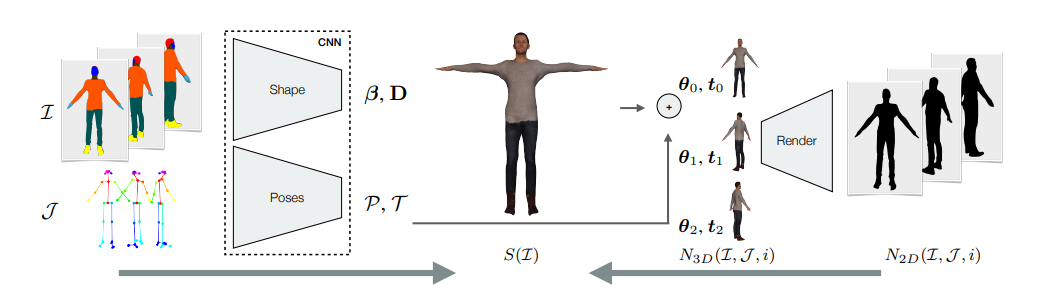
\includegraphics[width=0.95\textwidth]{fig/learningtoreconstruct.png}
    \caption{Learning to Reconstruct People in Clothing from a Single RGB Camera.~\cite{alldieck2019learningreconstructpeopleclothing}}
    \label{fig:learningto}
\end{figure}

To improve generalization and accuracy, multiple loss terms are used here. These include vertex-level reconstruction losses in both T-pose and posed configurations, 2D silhouette, 3D and 2D joint consistency, and regularization terms to constrain the undressed body shape. Notably, the method introduces a self-supervised refinement step at test time: by fixing most network weights and optimizing latent layers using 2D projections, the model can adapt to instance-specific geometry using only RGB inputs.

Overall, this approach demonstrates that fast, accurate reconstruction of animatable 3D human models is feasible from a small number of monocular frames, even in unconstrained settings. Its reliance on semantic cues and its top-down refinement capability make it particularly appealing for practical real-world deployment.

\subsection{Re-Identification Supervised Texture Generation}

Wang et al.~\cite{wang2019reidentificationsupervisedtexturegeneration} propose a texture generation framework guided by person re-identification supervision. The central idea is to train a texture generator by maximizing the perceptual similarity between the rendered person and the input image. This is achieved by comparing deep features extracted by a pre-trained person re-identification network.

The method starts by estimating SMPL parameters~\cite{SMPL:2015} using HMR~\cite{kanazawaHMR18}, which are then used to compute a 3D mesh. A U-Net~\cite{ronneberger2015unetconvolutionalnetworksbiomedical} is employed to generate the corresponding UV texture from the input image. This texture is rendered onto the 3D mesh using a differentiable renderer (OpenDR~\cite{opendr2022}), producing a synthetic image. The similarity between the input and rendered images is then enforced via a re-identification loss, which computes $\ell_2$ distances between features extracted from multiple layers of a PCB-based~\cite{sharma2021personreidentificationlocallyaware} person re-ID network.

\begin{figure}[h]
    \centering
    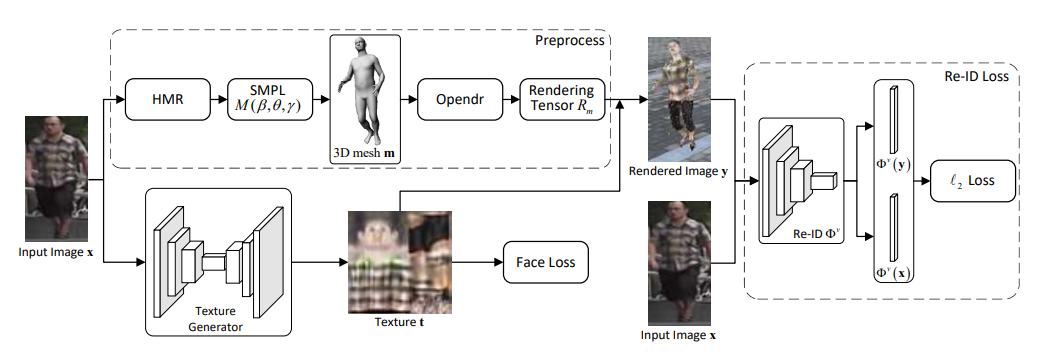
\includegraphics[width=0.95\textwidth]{fig/reid.png}
    \caption{Re-Identification Supervised Texture Generation.~\cite{wang2019reidentificationsupervisedtexturegeneration}}
    \label{fig:reid}
\end{figure}

In addition to the re-identification loss, a face-specific loss is introduced to enhance facial fidelity. This loss computes the $\ell_1$ distance between the generated and ground-truth textures (from the SURREAL dataset~\cite{varol17_surreal}) over face and hand regions, as defined by a semantic mask. Rather than pasting scanned face textures directly, this strategy ensures smooth color transitions across body parts and avoids visual artifacts.

The final training objective combines both terms:

\[
\mathcal{L} = \lambda_{\text{reid}} \mathcal{L}_{\text{reid}} + \lambda_{\text{face}} \mathcal{L}_{\text{face}},
\]

where the weights control the relative importance of identity preservation and facial realism. Notably, the use of a re-identification network for supervision aligns texture generation with human identity, enabling high-quality appearance synthesis that is consistent with the subject in the input image.



\subsection{TexDreamer}

TexDreamer~\cite{liu2024texdreamer} is the first zero-shot multimodal high-fidelity method for human texture generation in the SMPL UV space. It leverages large-scale pretrained Latent Diffusion Models (LDMs) and introduces a two-stage pipeline: Text-to-UV (T2UV) and Image-to-UV (I2UV).

To support training, the authors construct the ATLAS dataset, consisting of 50k high-resolution SMPL-compatible UV textures generated by UV projection and project-painting from multi-view images. Synthetic textures are enriched with animation (via AMASS~\cite{AMASS:ICCV:2019}), Physically Based Rendering(PBR) rendering, and diverse backgrounds, providing millions of rendering frames.

The \textbf{T2UV} module is fine-tuned from Stable Diffusion using LoRA~\cite{hu2022lora}, injecting a small number of trainable parameters into each attention layer. The fine-tuning objective modifies the LDM denoising loss as:
\begin{equation}
\mathcal{L}_{\text{T2UV}} = \mathbb{E}_{\mathcal{E}(x), c, \epsilon, t} \left[\left\|\epsilon - \phi_{\text{unet}}(z_t, t, \phi_{\text{tenc}}(c))\right\|^2\right],
\end{equation}
where $z_t$ is the noisy latent, $c$ the text prompt, and $\phi_{\text{unet}}$ the diffusion backbone.

The \textbf{I2UV} module bridges visual and textual domains by learning a feature translator from 2D image features (via CLIP~\cite{radford2021learningtransferablevisualmodels}) to the text embedding space of T2UV. The translated features condition the same denoising process used in T2UV:
\begin{equation}
\mathcal{L}_{\text{I2UV}} = \mathbb{E}_{\mathcal{E}(x), y, \epsilon, t} \left[\left\|\epsilon - \phi_{\text{unet}}(z_t, t, \phi_{i2t}(y))\right\|^2\right],
\end{equation}
enabling high-quality UV texture prediction from real images.

TexDreamer achieves strong semantic alignment and texture fidelity, enabled by structured prompt design, CLIP-based filtering, and semantic-aware conditioning. It sets a new direction in human texture generation by combining data-efficient adaptation with pretrained generative priors.


\begin{figure}[h]
    \centering
    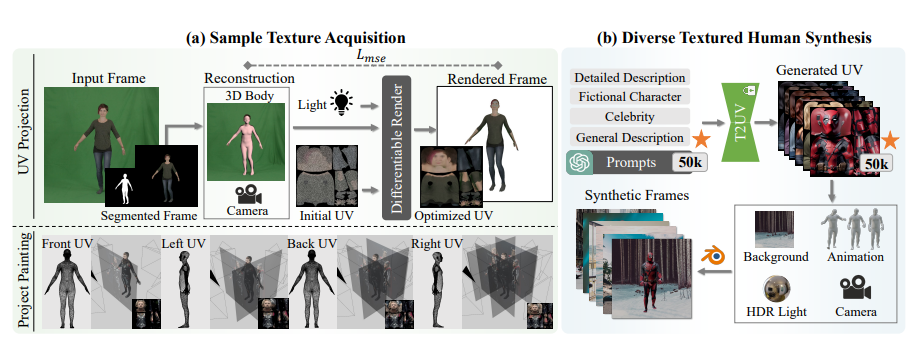
\includegraphics[width=0.95\textwidth]{fig/texdreamer.png}
    \caption{TexDreamer: Towards Zero-Shot High-Fidelity 3D Human Texture Generation Architecture.~\cite{liu2024texdreamer}}
    \label{fig:texdreamer}
\end{figure}

\subsection{Comparison and Summary}

\begin{table}[h]
\centering
\renewcommand{\arraystretch}{1.2}
\resizebox{\textwidth}{!}{ 
\begin{tabular}{l|c|c|c|c|c|c}
\toprule
\textbf{Method} & \textbf{Backbone} & \textbf{Input} & \textbf{Guidance} & \textbf{UV Format} & \textbf{Resolution} & \textbf{Notes} \\
\midrule
\textbf{SMPLitex} & Diffusion (LDM) & RGB + Partial UV & DensePose + SGHM & Full UV & $512^2$ & Generative prior \\
\textbf{Texformer} & Transformer & RGB + Segmentation & QKV Attention & Full UV & $512^2$ & Combines RGB + Flow \\
\textbf{HPBTT} & CNN & Human Parsing & Cross-view Flow & Full UV & $512^2$ & Supervision-free \\
\textbf{360-Texture} & CNN + GAN & Partial Texture & DensePose + SMPL reg. & Full UV & up to $512^2$ & GAN + I2I inpainting \\
\textbf{TexDreamer} & Diffusion (LDM) & Text / Image & Feature Translator & Full UV & $1024^2$ & Zero-shot, ATLAS dataset \\
\textbf{ReIDTex} & CNN + ReID & RGB & HMR + ReID Features & Full UV & $512^2$ & Optimized for identity similarity \\
\textbf{RGB-to-3D} & CNN + SMPL+D & Semantic Seg. + 2D Joints & 3D SMPL+D Regressor & Mesh $\to$ UV & -- & Fast, animatable mesh output \\
\bottomrule
\end{tabular}
}  
\caption{Comparison of recent human texture estimation and reconstruction methods.}
\end{table}






\section{Research Gap and Motivation for HRHumanTex}

Even with these works have made progress in human texture estimation, however, some key limitations still prevent its wider use in high-fidelity 3D reconstruction and animation processes.

\textbf{(1) Low Texture Resolution.}  
Many existing approaches, including SMPLitex~\cite{casas2023smplitex}, generate UV textures at a fixed resolution of $512{\times}512$, which limits their effectiveness in applications that require detailed surface quality, such as photorealistic digital humans or virtual try-on systems. While TexDreamer~\cite{liu2024texdreamer} expands to $1024^2$ resolution, its reliance on large-scale datasets (50,000 textures) and heavy pretraining pipelines makes it less accessible in data-scarce settings. It's a resource-intensive approach.

\textbf{(2) Data Scarcity and Generalization.}  
SMPLitex inpainting-based methods are trained on small datasets—sometimes fewer than 20 texture instances—which constrains the model's ability to generalize to unseen images. This often results in visible weird artifacts and hallucinations in generated textures.

\textbf{(3) Limited Evaluation Protocols.}  
Evaluation strategies in prior work are often narrowly focused on UV-space metrics or visual inspection. Few methods incorporate 3D rendering-based comparisons that assess how textures behave under realistic deformations and pose variation. Metrics that align with the geometric and perceptual structure of the human body—such as UV-aware SSIM or LPIPS computed on rendered outputs—remain not fully developed.

\medskip

\noindent
To address these challenges, this thesis introduces the High-Resolution Human Texture (HRHumanTex) estimation framework, which aims to improve resolution, robustness, and evaluation for human texture estimation. The proposed pipeline features and main contributions:

\begin{itemize}
    \item Integration of advanced super-resolution models to upscale $512{\times}512$ textures to $1024{\times}1024$ with minimal quality loss;
    \item Use of diffusion-based inpainting models to complete partial UV textures while preserving structural consistency;
    \item A comparative analysis of multiple super-resolution architectures at UV texture enhancement tasks;
    \item A comprehensive evaluation pipeline that combines UV-space metrics (PSNR, SSIM, LPIPS, and FID),rendering-based evaluation and rendering-based optimization.
\end{itemize}

By combining resolution upscaling, robust texture completion, and multi-level evaluation, HRHumanTex seeks to close the gap between limited-data scenarios and the high-quality requirements of modern 3D human applications.
